\documentclass{elegantbook}

\author{Miao}
\date{\today}
\email{chenmiao.ku@gmail.com}
\usepackage{ntheorem}
\zhtitle{考研OS学习}
\entitle{Exam OS Learning}
\enend{Note}
\version{0.10}
\myquote{Victory won\rq t come to us unless we go to it.}
\logo{ElegantLaTeX_green.pdf}
\cover{cover.pdf}

\usepackage{listings}
\usepackage{xcolor}
\usepackage{makecell}
\usepackage{lipsum}
\usepackage{texnames}
\usepackage{multirow}
% \usepackage{ulem}

\lstset{ 
  backgroundcolor=\color{white},   % 选择代码背景,必须加上\ usepackage {color}或\ usepackage {xcolor}.
  basicstyle=\small\bf,            % 设置代码字号.
  breakatwhitespace=false,         % 设置是否当且仅当在空白处自动中断.
  breaklines=true,                 % 设置自动断行.
  captionpos=b,                    % 设置标题位置.
  commentstyle=\color{red},        % 设置注释格式
  deletekeywords={...},            % 是否删除给定语言的关键词.
  escapeinside={\%*}{*)},          % 是否在代码中添加LaTex.
  extendedchars=true,              % 是否允许使用非ASCII字符; 仅适用于8位编码,不适用于UTF-8. 
  frame=single,	                   % 给代码区添加边框.
  keepspaces=true,                 % 保留空格(useful for keeping indentation of code (possibly needs columns=flexible).
  keywordstyle=\color{blue},       % 关键字显示风格.
  language=C++,                    % 使用的语言.
  morekeywords={*,...},            % 是否需要添加其他的关键词.
  numbers=left,                    % 给代码添加行号,可取值none, left, right.
  numbersep=5pt,                   % 设置行号与代码之间的间隔
  numberstyle=\bf\color{blue},     % 行号的字号和颜色
  rulecolor=\color{black},         % 边框颜色,如果没有设置,框架颜色可以在非黑色文本中的换行符上更改(例如 text (e.g. comments (green here)))
  showspaces=false,                % 显示每个地方添加特定下划线的空格; 覆盖了'showtringspaces'
  showstringspaces=false,          % 仅在字符串中允许空格
  showtabs=false,                  % show tabs within strings adding particular underscores
  stepnumber=2,                    % the step between two line-numbers. If it's 1, each line will be numbered
  stringstyle=\color{blue},       % string literal style
  tabsize=4,	                     % 将默认tab设置为2个空格
  title=\lstname                   % show the filename of files included with \lstinputlisting; also try caption instead of title
}

\begin{document}
    \maketitle
    \tableofcontents
    \chapter{绪论}

\section{操作系统基本概念}

    \emph{任何计算机系统都包含一个名为操作系统的基本程序集合。}在这个集合中,最重要的程序称为内核(kernel)。启动后,内核中包含了系统运行所必不可少的很多核心过程(procedure),和其他一些不太重要的实用程序。

    \emph{系统根本的样子和能力还是由内核决定,内核也为操作系统中所有事情提供了主要功能,并决定高层软件的很多特性。}

    操作系统必须完成两个主要目标:

\begin{itemize}
    \item [1)] 与硬件部分交互,为包含在硬件平台上的所有底层可编程部件提供服务
    \item [2)] 为运行在计算机系统上的应用程序提供执行环境
\end{itemize}

    \emph{类Unix系统把与计算机物理组织相关的所有底层细节都对用户运行的程序隐藏起来,硬件为CPU引入了至少两种不同的执行模式:非特权模式(用户态(User Mode)和特权模式(Kernel Mode))}。

\section{多用户系统}

    \emph{多用户系统(multiuser system)就是一台能并发和独立地执行分别属于两个或多个用户的若干应用程序的计算机。}

    并发(concurrently)意味着几个应用程序能够同时处于活动状态并竞争各种资源。独立(independently)意味着每个应用程序能够执行自己的任务,而无需考虑其他用户的应用程序在做什么。

    多用户操作系统必须包含:

\begin{itemize}
    \item [1)] 核实用户身份的认证机制
    \item [2)] 防止有错误的用户程序妨碍其他应用程序在系统中运行的保护机制
    \item [3)] 防止有恶意的用户程序干涩或窥视其他用户的活动的保护机制
    \item [4)] 限制分配给每个用户的资源数的记账机制
\end{itemize}

\section{用户和组}

    操作系统必须保证用户空间的私有部分仅仅对于其拥有者是可见的。

    所有的用户由一个唯一的数字来表示,这个数字叫用户标识符(User ID, UID)。

    为了和其他用户有选择地共享资料,每个用户是一个或多个用户组的一名成员,组由唯一的用户组标识符(user group ID)标识。每个文件也恰好与一个组相对应。

    \emph{任何类Unix操作系统都有一个特殊的用户,root(超级用户(superuser))}。系统管理员能够通过root账号登陆,值得一提的是:\emph{root几乎无所不能,其能访问系统中的每一个文件,能干涉每一个正在执行的用户程序}。

\section{进程}

    \emph{所有的操作系统都有一种基本的抽象:进程(process)。一个进程可以定义为:"程序运行时的一个实例",或者一个运行程序的"执行上下文"}。

    传统的操作系统中,\emph{一个进程在地址空间中(address space)执行一个单独的指令序列。}现代操作系统允许具有多个执行流的进程,也就是在相同的地址空间可执行多个指令序列。

    \emph{允许进程并发活动的系统称为多道程序系统(multiprogramming)或多处理系统(multiprocessing)}。值得注意的是:几个进程能够并发地执行同一个程序,而同一个进程能顺序的执行几个程序。

    调度程序(scheduler)的部分决定哪个进程能执行,一些操作系统只允许有非抢占式(nonpreemptable)进程,\emph{也就是说,只有当进程自愿放弃时,调度程序才能被调用。但是,多用户系统中的进程必须是抢占式的(preemptable)}。

\section{内核体系结构}

    大部分Unix内核都是单块结构:\emph{每一个内核层都被集成到整个内核程序中,并代表当前进程在内核态下运行。}

    \emph{微内核(microkernel)操作系统只需要内核有一个很小的函数集(几个同步原语\footnote[1]{原语(primitive)是计算机科学中的一个概念,它指的是一组基本的操作或指令,可以直接在计算机硬件上执行。原语通常是由计算机硬件提供的,用于支持高级编程语言或操作系统的功能},一个简单的调度程序和进程间通信)}。

    Linux内核提供了模块(module)用于达到微内核理论上的很多优点且不影响性能。\emph{模块是一个目标文件,其代码可以在运行时链接到内核或从内核解除链接。这种目标代码通常由一组函数组成,用来实现文件系统、驱动程序或其他内核上层功能。}

    使用模块的主要优点:

\begin{itemize}
    \item [1)] 模块化方法
    \subitem 任何模块都能在运行时被链接或解除链接。这要求程序员提出良定义的软件接口以访问由模块处理的数据结构
    \item [2)] 平台无关性
    \subitem 即使模块依赖于某些特殊的硬件特点,但它不依赖于某个固定的硬件平台
    \item [3)] 节省内存使用
    \subitem 当需要模块时,就链接;不需要时,则解除
    \item [4)] 无性能损失
    \subitem 模块的目标代码一旦被链接进内核,起作用与静态链接的内核的目标代码完全对等。因此无需显式的进行消息传递\footnote[1]{模块被链接或解除时,都有一定的性能下降。但是在微内核中也是如此}
\end{itemize}

\section{Unix文件系统概述}

\subsection{文件}

    \emph{Unix文件是以字节序列组成的信息载体(container),内核不解释文件的内容。}

    从用户的观点来看,文件被组织在一个树结构的命名空间内:

\begin{figure}[!htbp]
    \centering
    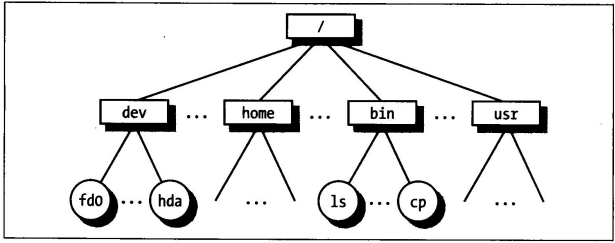
\includegraphics[width=0.6\textwidth]{image/chapter01/目录树结构.png}
    \caption{目录树结构}
\end{figure}

    除叶节点外,所有节点都表示目录名。目录节点包含它下面文件及目录的所有信息。

    \emph{Unix每个进程都有一个当前工作目录,属于进程执行上下文(execution context),标识出进程所用的当前目录。}

    \emph{路径名(pathname)由斜杠及一列指向文件的目录名交替组成。如果第一个字符是斜杠,那么就是所谓的绝对路径;否则就是所谓的相对路径。}

    当标识文件名时,用符号"."和".."分别标识当前工作目录和父目录。

\subsection{硬链接和软连接}

    \emph{包含在目录中的文件名就是一个文件的硬链接(hard link),或简称连接(link)。}

    使用Unix命令:

\begin{lstlisting}[language=C++]
$ ln P1 P2
\end{lstlisting}

    用来创建一个新的硬链接,即为由路径P1标识的文件创建一个路径名为P2的硬链接。

    硬链接有两方面的限制:

\begin{itemize}
    \item [1)] 不允许给目录创建硬链接,这可能使得目录树编程环形图从而无法通过名字定位一个文件
    \item [2)] 只有在同一文件系统中的文件之间才能创建链接。
\end{itemize}

    为了克服限制,引入\emph{软链接(soft link)[也称符号链接(symbolic link)],符号链接是短文件,这些文件包含另一个文件的任意一个路径名。}

    值得注意的是:\emph{路径名可以指向位于任意一个文件系统的任意文件或目录(哪怕它不存在)}。

    Unix命令:

\begin{lstlisting}[language=C++]
$ ln -s P1 P2
\end{lstlisting}

    创建一个路径名为P2的新软连接,P2指向路径名P1。当执行命令时,文件系统抽取P2的目录部分,并在此创建P2的符号链接属性的新项。因此,任何对P2的引用都可以自动被转换为指向P1的引用。

\subsection{文件类型}

    Unix命令文件可以是以下类型:

\begin{itemize}
    \item 普通文件(regular file)
    \item 目录
    \item 符号链接
    \item 面向块的设备文件(block-oriented device file)
    \item 面向字符的设备文件(character-oriented device file)
    \item 管道(pipe)和命名管道(named pipe)(也叫FIFO)
    \item 套接字(socket)
\end{itemize}

\subsection{文件描述符与索引节点}

    \emph{除了设备文件和特殊文件系统外,每个文件都由字符序列组成。文件内容不包括任何控制信息,如文件长度或文件结束符(end-of-file, EOF)}。

    \emph{文件系统处理文件需要的所有信息都包含在一个名为索引节点(inode)的数据结构中,文件系统用索引节点来标识文件。}

    索引节点(inode)至少包括:

\begin{itemize}
    \item 文件类型
    \item 与文件相关的硬链接个数
    \item 以字节为单位的文件长度
    \item 设备标识符(即包含文件的设备的标识符)
    \item 文件系统中标识的索引节点号
    \item 文件拥有者的UID
    \item 文件的用户组ID
    \item 几个时间戳(改变时间、最后访问时间、最后修改时间)
    \item 访问权限和文件模式
\end{itemize}

\subsection{访问权限和文件模式}

    文件的潜在用户分为三种类型:

\begin{itemize}
    \item 文件所有者
    \item 同组用户(不含所有者)
    \item 其他用户
\end{itemize}

    同时,拥有三种类型的访问权限————读、写以及执行。因此就有九种组合不同的二进制来标记,还有三种额外的标记

\begin{itemize}
    \item suid
    \subitem 进程执行一个文件时通常保持进程拥有者的UID,若设置suid,进程就可以获取该文件拥有者的UID
    \item sgid 
    \subitem 进程执行一个文件时保持进程组的用户组ID,若设置sgid,进程就可以获得该文件用户组ID
    \item sticky
    \subitem 设置sticky标志位相当于向内核发出请求,当程序结束后仍保留在内存\footnote[1]{该标记已经过时,已被其他方法取代}
\end{itemize}


\end{document}
